%--------------------------------------------------------------------------- % Chapter 2 - Similar technologies %

%--------------------------------------------------------------------------- 
\section{Overview of similar monitoring systems} \label{sec:ch2_similar}

%---------------------------------------------------------------------------

\subsection{perfSonar}

The perfSONAR (\cite{perfSonar1,perfSonar2,perfSonar3}) is an infrastructure for network performance monitoring. It aims in making process of solving end-to-end performance problems on paths crossing several networks easier. It is composed of a set of services delivering performance measurements in a federated environment. This approach allows classification of project as a middle ware service that is in use by performance measuring tools and diagnostic or visualization applications. The perfSonar layer tries to generate and exchange measurement data between networks. It performs communication using well defined protocols. Architecture of perfSONAR is service oriented, which means that the set of elementary functions (\emph{services}) has been isolated and can be provided by several, independent entities.

Work done on perfSONAR is made around three contexts. First, there is a consortium of organizations that build a network of performance middle ware that is interoperable across multiple networks and useful for a variety of network analysis. The second context is a protocol. It is built on an assumption of fixed, well defined roles (service types) and defines communication model between components implementing each role. Well defined Protocol is the most important mean to achieve interoperability. What is also worth mentioning, proposed protocol is based on SOAP XML messages format and follows Network Measurement Working Group\footnote{\url{http://nmwg.internet2.edu}} schema. The third context is set of implemented software packages that provide services mentioned above.

The framework defines following types of services:

\begin{itemize}

\item{ {\bf Measurement Point Service} acts as a service provider. Standard does not define whether it gathers measurement values dynamically, by querying measured components or retrieves static, archived data. It defines only role of this component as a source of measurement values.}

\item{ {\bf Measurement Archive Service} is responsible for archiving data. It can use any storage facility underneath (Round Robin Database or any other RDBMS). Additionally it can publish received information. }

\item{ {\bf Lookup Service} enables services to discover each other. It acts as service directory, where providers can advertise themselves and requesters are able to find any service needed}

\item{ {\bf Authentication Service} helps domains which would like to restrict access to given service capabilities for some groups of users. It is responsible for both authorization and authentication. It acts as, so called, attribute authority which decides which attribute can be disclosed to a resource}

\item{ {\bf Transformation Service} is a generic service type that allows creation of data conversion pipelines. It can perform any function upon data taken from a producer and return transformed data to a consumer}

\item{ {\bf Topology Service}, provides the framework information about network topology, which allows, for example, visualization of network maps. Additionally it gives information on geolocation, like GPS coordinates.}

\item{ {\bf Resource Protector Service} - it is used to arbitrate the consumption of limited, shared resources, e.g. network bandwidth} \end{itemize}

%---------------------------------------------------------------------------

\subsection{SCALEA and SCALEA-G}

SCALEA~\cite{SCALEA1} is a tool for instrumentation, measurement, analysis and visualization of parallel programs execution. It can work with OpenMP, MPI, HPF, and mixed parallel/distributed systems. Its measurements are based on a variety of performance metrics, but SCALEA also supports multiple experiment performance analysis that allows to compare and to evaluate the performance outcome of several experiments.

Architecture of system distinguishes three main components: SCALEA Instrumentation System (\emph{SIS}), SCALEA Runtime System (\emph{SRS}) and SCALEA Performance Analysis \& Visualization System. SIS can instrument any of FORTRAN, OpenMP, MPI, HPF or even hybrid programs like OpenMP/MPI and allows the user to select code regions and performance metrics of interest. Using this input, SIS inserts probes in the code which will collect all relevant performance information. Those data are saved in a set of profile (trace) files during program execution, which is monitored by SRS. Additionally, SIS component is responsible for generation of instrumentation description file that can be used to associate gathered performance data back to the input program. Performance Analysis \& Visualization sub system can use raw data gathered either during the program execution or post-mortem.

The main purpose of SCALEA-G (\cite{SCALEA2, SCALEA3}) is to bring functionality of SCALEA to the grid environment. Originally it was implemented as a set of OGSA services based on Globus Toolkit 3.0, but it was ported then into WSRF-based services with Globus Toolkit 4.0. The most recent implementation of SCALEA-G is composed of following services:

\begin{itemize}

\item{ {\bf Registry Service}}

\item{ {\bf Directory Service}}

\item{ {\bf Sensor Manager Service} - monitors and measures performance of Grid services. Internally, it is implemented as WSRF-based service that collects monitoring data from sensors. It supports 2 communication modes - both query/request and subscribe/notify. Collected data are stored in XML containers, based on DBXML.}

\item{ {\bf Dynamic Instrumentation Service}, used for instrumentation of native application. It uses internally C++ gSOAP+, GSI-plugin and Dyninst.}

\item{ {\bf XML data schema Service}}

\item{ {\bf Client Service}}

\item{ {\bf GUI Component}}

\item{ {\bf Set of Java APIs}}

\end{itemize}

%---------------------------------------------------------------------------

\subsection{DIPAS}

DIPAS~\cite{DIPAS}, which stands for Distributed Performance Analysis Service, is a monitoring platform designed to work with K-WfGrid (see section~\ref{ssec:kwfgrid}). The aim of this project is to provide on-line information about the performance of Grid workflows as well as Grid resources involved in the execution process. Those data are used not only by the user, but also by the K-WfGrid middle ware and services, they are a source of knowledge about the performance, which improves the process of semi-automatic workflow construction.

DIPAS provides performance analysis and interpretation for workflows which is based on a novel classification of performance overheads. It allows the user to define the performance constraints. Later, using this input, DIPAS informs the user and client about potential performance problems by interpreting metrics at runtime. Performance analysis of workflows is integrated with tools built-in to the Grid infrastructure, creating coherent framework.

Additionally, DIPAS provides a web portal for the user to conduct performance monitoring and analysis of workflows with underlying infrastructure. These components substantially simplifies the way that a user interacts with the tool.

Overall architecture of the system is outlined in Figure~\ref{fig:dipas}

\begin{figure}[ht]

\centering

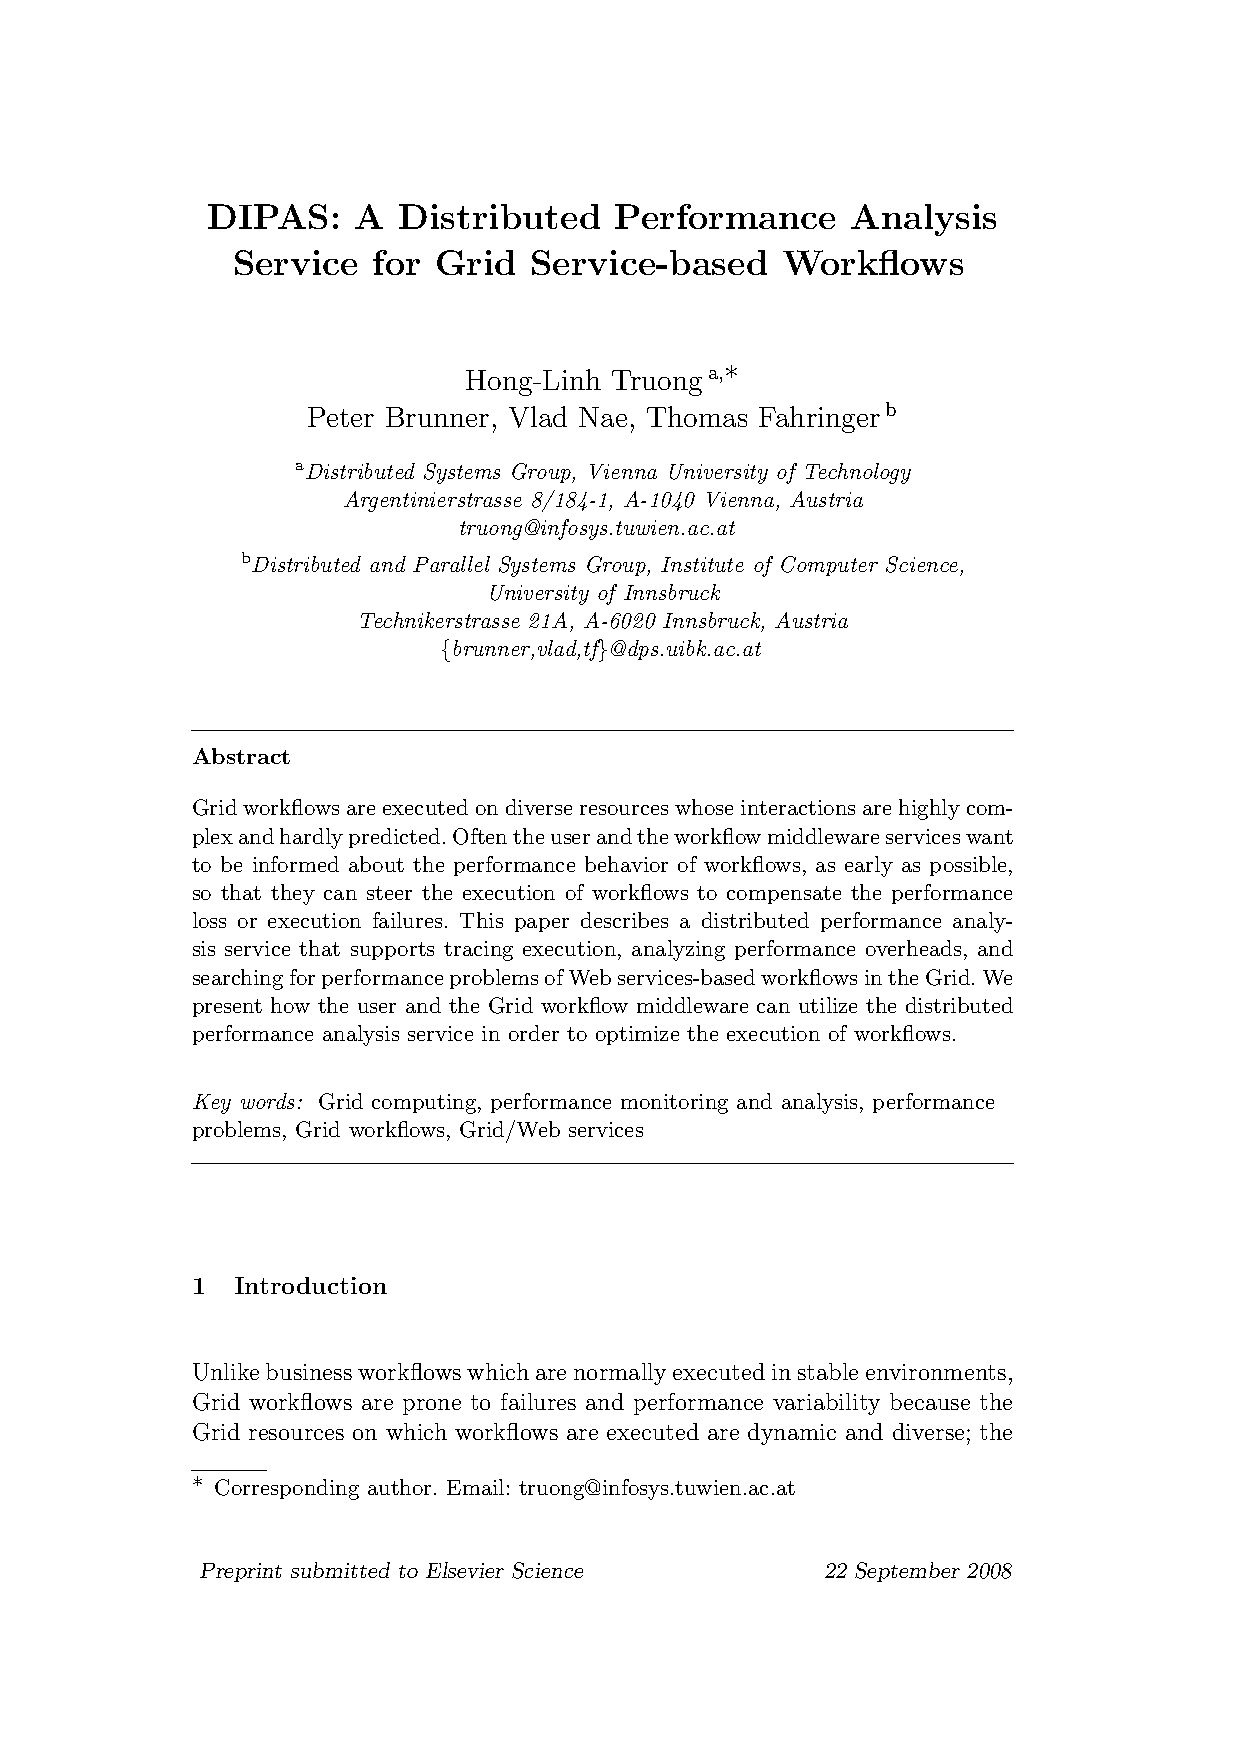
\includegraphics[width=0.6\textwidth]{dipas} \caption{Overall architecture of DIPAS} \label{fig:dipas}

\end{figure}

%---------------------------------------------------------------------------

\subsection{OCM Family}

As part of work on OMIS (See section~\ref{ssec:omis}), several tools that are compliant with this interface were introduced. This tool set includes OCM\footnote{\url{http://www.lrr.in.tum.de/Par/tools/Projects/OCM.html}}, OCM-G\footnote{\url{http://grid.cyfronet.pl/ocmg}}, JOCM\footnote{\url{http://jocm.icsr.agh.edu.pl/sub/main}} and G-PM\footnote{\url{http://gpm.icsr.agh.edu.pl}}.

OCM (\cite{RWspdt98, RW:ppam99b}) - OMIS Compliant Monitoring System is the first tool in a whole set. The main goal of this project was to create a reference implementation of an OMIS compliant monitoring system. Initially it has been supporting PVM (versions 3.3 and 3.4) and MPI-1.

As a next step in platform evolution, OCM-G (\cite{axgrid03b}) was introduced. Name of the project is an abbreviation for Grid-enabled OMIS-Compliant Monitoring system. This project focuses on using OMIS interface with grid environment. In spite of working with well-known MPI parallel programming library, it was designed to work with Globus Toolkit and is fully compliant with EGEE environment including gLite 3.x\footnote{\url{http://glite.cern.ch/}} and LCG 2.7.

The latest addition to the set of OMIS-compliant tools is JOCM - Java oriented monitoring infrastructure (\cite{jocm}). It adds the ability of monitoring JVM based applications. It has extended OMIS interface with a set of new, specific for Java services, like garbage collection, threads execution, class loading or method invocation. Currently project implementation focuses on monitoring Java Web Services and component oriented applications.

General architecture shared among all mentioned above implementations can be found in Figure~\ref{fig:ocmg}.

\begin{figure}[ht]

\centering

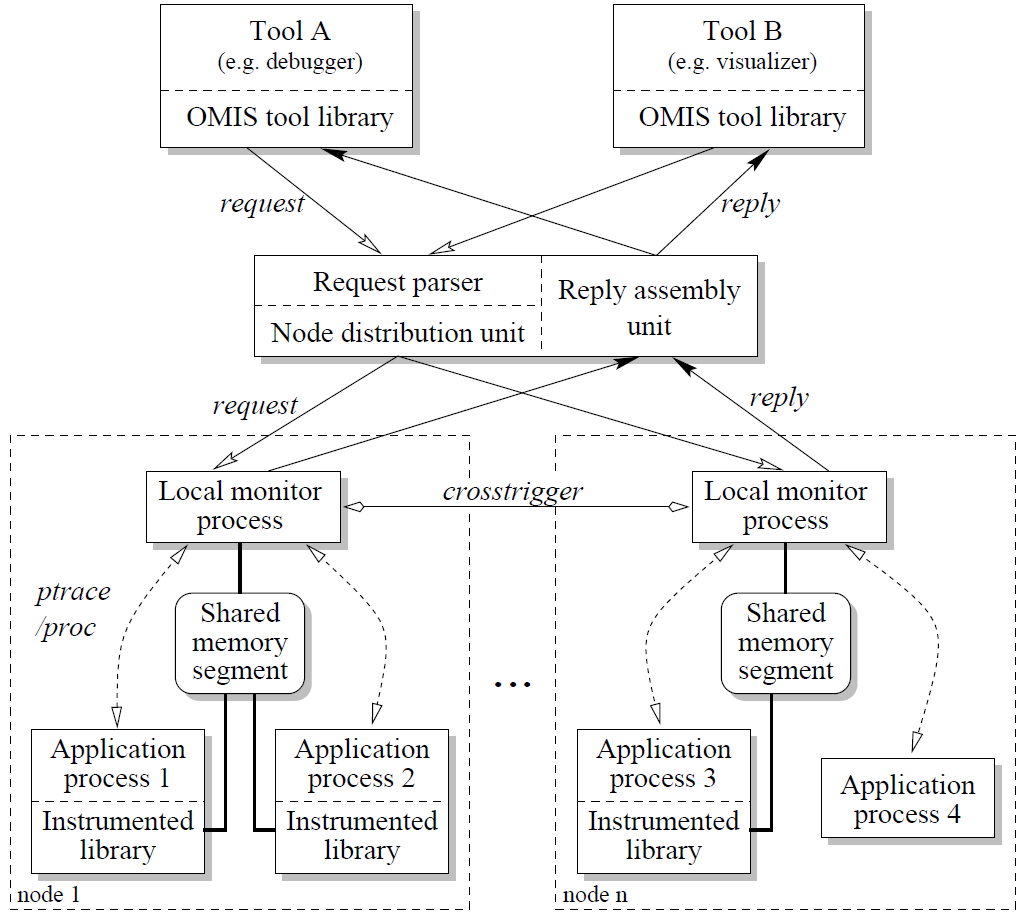
\includegraphics[width=0.8\textwidth]{ocm_arch} \caption{Common OMIS-compliant tools architecture diagram} \label{fig:ocmg}

\end{figure}

%---------------------------------------------------------------------------

\subsection{R-GMA}

R-GMA: Relational Grid Monitoring Architecture~(\cite{RGMA1,RGMA2,RGMA3}) is implementation of GMA, described in section~\ref{ssec:gma}. Although it implements GMA interface, it adds two exceptions to the standard. First, anyone supplying or obtaining information from R-GMA does not need to know about the Registry component, as its responsibility is processed by Consumer and Producer components \lq\lq{}behind the scenes\rq\rq{}. The second exception is that information and monitoring system appears to the end user, like one large relational database and can be queried as such. It is the source of "R" (Relational) in the project name.

All systems that use R-GMA, share information in a virtual database. Data in this database are organized into tables and are managed with the help of standard SQL constructs (like INSERT INTO... or SELECT FROM). With regard to an internal database structure, there is no such thing as a central repository, which holds the data for each table. Virtual database just contains a list of table definitions (\emph{schema}), a list of data providers (\emph{registry}) and a set of rules for deciding which data provider needs to be used while preparing result for given query. These rules are fixed and encoded into an internal component called \emph{mediator}.

The system provides several ways to access the database. There is provided API, with bindings available in Java, C/C++ and Python. Additionally users can work with the database using the web interface or command line utility.